\documentclass[10pt,xcolor=pdflatex]{beamer}
\usepackage{newcent}
\usepackage[utf8]{inputenc}
\usepackage[czech]{babel}
\usepackage{hyperref}
\usepackage{fancyvrb}
\usetheme{FIT}
\usepackage{booktabs}
\usepackage{multirow}
\usepackage{amsmath}
\usepackage{cellspace}
\usepackage{regexpatch}
\usepackage{array}
\usepackage{tabularx}
\usepackage{graphicx}

%\ifczechslovak
  \makeatletter
  % Change the `-` delimiter to an active character
  \xpatchparametertext\@@@cmidrule{-}{\cA-}{}{}
  \xpatchparametertext\@cline{-}{\cA-}{}{}
  \makeatother
%\fi
%%%%%%%%%%%%%%%%%%%%%%%%%%%%%%%%%%%%%%%%%%%%%%%%%%%%%%%%%%%%%%%%%%

\title[Detekce akustického prostředí z audio nahrávek]{Detekce akustického prostředí z audio nahrávek}

%\author[]{Filip Grepl}
\author{Filip Grepl\\  {\footnotesize Vedoucí: Ing. Pavel Matějka, Ph.D. }}
\institute[]{Vysoké učení technické v Brně, Fakulta informačních technologií\\
Bo\v{z}et\v{e}chova 1/2. 612 66 Brno - Královo Pole\\
xgrepl05@stud.fit.vutbr.cz}


\date{Červen 12, 2018}
%\date{\today}
%\date{} % bez data

%%%%%%%%%%%%%%%%%%%%%%%%%%%%%%%%%%%%%%%%%%%%%%%%%%%%%%%%%%%%%%%%%%

\begin{document}


%\begin{columns}[b]
%\column{6cm}
%\begin{itemize}
% \item 1
% \item 2
%\end{itemize}
%\column{6cm}
%\begin{center}
%			\scalebox{0.3}{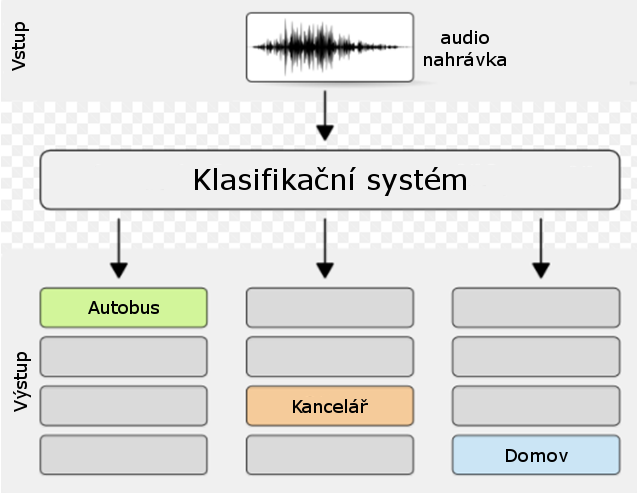
\includegraphics{img/cil_prace.png}}
   			%\caption{\textit{Prvý tlačiarenský lis}}
%		\end{center}
%\end{columns}

%Dobrý den, mé jméno je Filip Grepl a rád bych Vás seznámil se svou bakalářskou prací na téma Detekce akustického prostředí z audio nahrávek.

\frame[plain]{\titlepage}

%Nejprve by bylo vhodné si říct, co bylo cílem mé práce. Jak již samotý název napovídá, cílem mé práce bylo vytvořit systém, který dokáže ze vstupní audio nahrávky určit, na jakém místě byla tato audio nahrávka pořízena, přičemž se předpokládá, že pochází z jednoho z předem definovaných míst. Samotný klasifikátor jsem měl implementovat pomocí neuronové sítě.

\begin{frame}\frametitle{Cíl práce}

	\begin{figure}[ht]
		\begin{center}
			\scalebox{0.6}{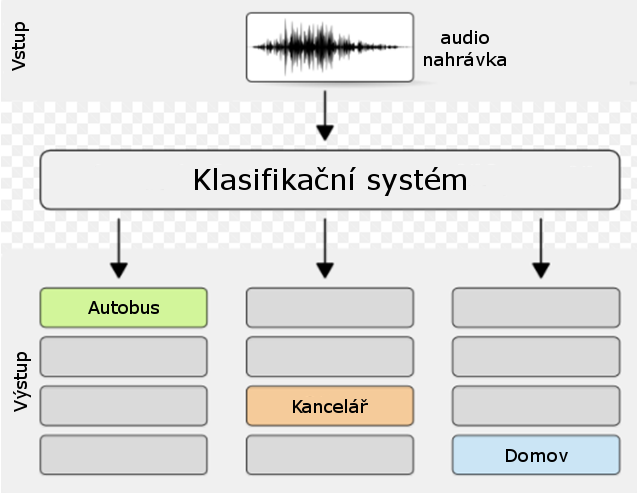
\includegraphics{img/cil_prace.png}}
		\end{center}
	\end{figure}
\end{frame}

%Pro trénování a evaluaci neuronové sítě jsem využíval datovou sadu, která byla poskytnuta k prvním úkolu soutěže DCASE v roce 2017, zabývajícímu se stejnou problematikou jako já ve své práci. Nahrávky v této sadě jsou z celkem 15ti míst, přičemž je každá z nich dlouhá 10 sekund. Z každého místa bylo pořízeno 312 nahrávek, celkem se jich tedy v datové sadě nachází 4680. Záznamy byly pořizovány ve stereo kvalitě se vzorkovací frekvencí 44.1 kHz a s rozlišením 24 bitů.

%\emph{content}.
\begin{frame}\frametitle{Datová sada DCASE 2017}    
    \begin{itemize}
    	\item Celkem 15 různých míst
    	\item Z každého místa 312 nahrávek, dohromady 4680 nahrávek
    	\item Každá nahrávka je dlouhá 10 s
    	%\item Vzorkovací frekvence 44.1 kHz, rozlišení 24 bitů
    \end{itemize}
	\begin{table}[H]
		\centerline 
		{
      		\begin{tabular}{l|l|l}
      			\toprule
           		\multicolumn{3}{c}{Tabulka klasifikačních míst} \\
        		\midrule
				Pláž				& Lesní cesta 			& Kancelář 		\\
				Autobus 			& Obchod s potravinami 	& Park 			\\
				Kavárna/Restaurace 	& Domov					& Obytná oblast	\\
				Auto				& Knihovna				& Vlak			\\
				Centrum města		& Stanice metra			& Tramvaj		\\
				\bottomrule
      		\end{tabular}
      	}
      %\caption{ Tabulka klasifikačních míst}
	\end{table}
\end{frame}


% Pro reprezentaci vlastností audio nahrávek jsem použil standardní Mel-filter bank a MFCC koeficienty, jelikož s nimi dosáhli soutěžící v již zmíněné soutěži DCASE nejlepších výsledků. Klasifikátor je realizován pomocí vícevrstvé hustě propojené neuronové sítě. Po mnoha provedených experimentech je výsledná topologie tvořena 2 skrytými vrstvami, přičemž obě obsahují 200 neuronů s aktivační funkcí ReLu a 2 vrstvami Dropout.

\begin{frame}\frametitle{Způsob řešení}
Reprezentace vlastností audio nahrávek:
\begin{itemize}
	\item Mel-filter bank (MFB)
		\begin{itemize}
			\item blok Mel-filter bank
		\end{itemize}
	\item Mel-frequency cepstral coefficients (MFCC)
\end{itemize}
Klasifikátor realizován pomocí vícevrstvé hustě propojené neuronové sítě
	\begin{table}[H]
		\centerline 
		{
      		\begin{tabular}{c}
      			\toprule
           		Vstupní vrstva 		\\
        		\midrule
				Dense(ReLu, 200) 	\\
				Dropout(0.2) 		\\
				Dense(ReLu, 200)	\\
				Dropout(0.2)		\\
				\midrule
				Dense(Softmax, 15)	\\
				\bottomrule
      		\end{tabular}
      	}
      %\caption{ Topologie neuronové sítě}
	\end{table}
\end{frame}

% Základní systém, který jsem postavil, byl trénován na MFB koeficientech získaných z původního audio signálu, který byl převzorkován na 8 kHz. Prováděl jsem experimenty s oběma kanály audio nahrávek, s normalizací vstupních dat i s rozšířením trénovací sady. Největšího zlepšení jsem však dosáhl při ponechání původní vzorkovací frekvence, kdy se úspěšnost zvýšila o celých 6 %. 

%\begin{frame}\frametitle{Experimenty s MFB koeficienty}
%	\begin{figure}[ht]
%		\begin{center}
%			\scalebox{0.6}{\includegraphics{img/%MFB_sampling_rate.eps}}
%		\end{center}
%	\end{figure}
%\end{frame}

% Následně jsem se zaměřil na blokové zpracování MFB koeficientů.  %Zkoušel jsem měnit jak velikost kontextu rámců, tak i počet příznaků reprezentujících jeden blok jednoho filtru.


%Při použití MFB koeficientů mi nejvíce pro zvýšení přesnosti klasifikace pomohlo jejich blokové zpracování. Nejprve jsem zkoušel experimentovat s velikostí kontextu rámců a s velikostí vektoru reprezentujícího jeden rámec audio signálu. Nejlepších výsledků jsem dosáhl s kontextem 10 rámců vlevo a 10 rámců vpravo od aktuálního rámce. S tímto nastavením jsem po té ještě zkoušel měnit počet trojúhelníkových filtrů. Jak můžete z tohoto grafu vidět, tak bylo nejvyšší úspěšnosti, 67.1 %, dosaženo se 46 trojúhelníkovými filtry. Další zvyšování jejich počtu už vedlo k horším výsledkům.
\begin{frame}\frametitle{Blok MFB koeficienty}
	\begin{figure}[ht]
		\begin{center}
			\scalebox{0.6}{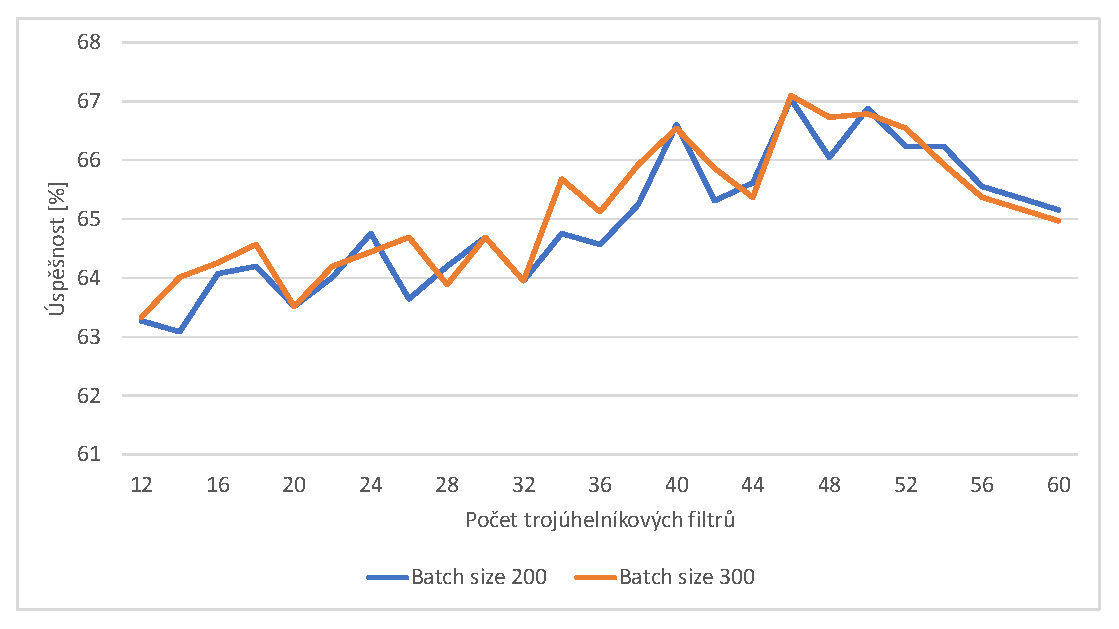
\includegraphics{img/number_MFB_filters_accurancy.eps}}
		\end{center}
	\end{figure}
\end{frame}

% Druhými příznaky, se kterými jsem experimentoval, byly MFCC koeficienty. Použil jsem pro ně 46 trojúhelníkových filtrů, jelikož jsem v předchozím experimentu s tímto počtem dosáhl nejlepších výsledků. Většinou se pro trénování neuronové sítě využívá pouze první polovina MFCC příznaků, nicméně z grafu je zřejmé, že bylo dosaženo nejvyšší přesnosti klasifikace, tj. 65 %, když se počet MFCC koeficientů rovnal počtu filtrů. Po přidání delta koeficientů se výsledná úspěšnost zvýšila o dalších 0.5 %.


% Dále již tento počet nebylo možné zvyšovat, jelikož počet MFCC příznaků musí být menší, než počet filtrů.

%\begin{frame}\frametitle{Experimenty s MFCC koeficienty}
%	\begin{figure}[ht]
%		\begin{center}
%			\scalebox{0.6}{\includegraphics{img/%number_MFCC_coefficients_accurancy.eps}}
%		\end{center}
%	\end{figure}
%\end{frame}

%Můj nejlepší systém byl natrénován ve 100 iteracích s parametrem batch size o velikosti 300 na blok MFB koeficientech s nastavením, které jsem vám již popsal. Tyto příznaky byly získané z  průměrné hodnoty obou kanálů, které byly ponechány na původní vzorkovací frekvenci 44.1 kHz. Způměrovaný signál byl rozdělen na rámce o velikosti 20 ms s překrýváním 60 %.

\begin{frame}\frametitle{Nejlepší systém}
	\begin{itemize}
		\item Původní vzorkovací frekvence 44.1 kHz
		\item Průměrná hodnota obou kanálů
		\item blok MFB koeficienty s kontextem 10 rámců 
		\item 46 trojúhelníkových filtrů
		\item žádná normalizace
	\end{itemize}
	\begin{table}[H]
		\centerline 
		{
      		\begin{tabular}{l|c}
      			\bottomrule
      			Parametr & Hodnota \\
      			\midrule
      			Délka rámce			& 20 ms				\\
				Překrývání			& 12 ms				\\
				Learning rate		& $1*10^{-5}$		\\
				Počet iterací		& 100				\\
				Batch size			& 300 				\\
				\bottomrule
      		\end{tabular}
      	}
	\end{table}
\end{frame}

% Jak jsem již zmínil, všechny experimenty jsem prováděl na datové sadě z roku 2017. Pro srovnání, jak se můj nejlepší systém chová na jiné množině dat, jsem však využil i datovou sadu z roku 2016. Výsledky můžete vidět na tomto slidu, kde jsem si připravil srovnání svého nejlepšího systému s oběma baseline systémy. Při použití datové sady z roku 2016 jsem dosáhl celkového zlepšení 5.9 %, s datovou sadou z roku 2017 pak 6.5 %. Z celkového počtu 41 týmů by se tak tento klasifikátor umístil na 12. místě.

\begin{frame}\frametitle{Porovnání výsledků}

\setlength\cellspacetoplimit{2pt}
\setlength\cellspacebottomlimit{2pt}
\newcolumntype{?}{!{\vrule width 1pt}}
\begin{table}[h]
\centerline {
\resizebox{\textwidth}{!}{%
	\begin{tabular}{Sc|Sc|Sc?Sc|Sc}
    	\bottomrule
          \multirow{4}{*}{Třída} & \multicolumn{4}{c}{Úspěšnost [\%]} \\ \cline{2-5}
          & \multicolumn{2}{Sc?}{Datová sada DCASE 2016} & \multicolumn{2}{Sc}{Datová sada DCASE 2017} \\ \cline{2-5}
          & \shortstack[c]{Základní systém\\ 2016} & \shortstack[c]{Nejlepší\\ systém} & \shortstack[c]{Základní systém\\ 2017} & \shortstack[c]{Nejlepší\\ systém} \\
        \midrule
		 		autobus   				&	88.5	&	96.2	&	38.9	&	43.5	\\	\hline		
              	knihovna				&	26.9	&	53.8	&	30.6	&	62.0	\\	\hline
              	kavárna/restaurace		&	69.2	&	61.5	&	43.5	&	59.3	\\	\hline
              	stanice metra			&	100.0	&	76.9	&	93.5	&	100.0	\\	\hline
              	auto					&	96.2	&	100.0	&	64.8	&	71.3	\\	\hline
              	kancelář				&	96.2	&	100.0	&	73.1	&	63.0	\\	\hline
              	centrum města			&	80.8	&	84.6	&	79.6	&	92.6	\\	\hline
              	obytná oblast			&	88.5	&	65.4	&	77.8	&	85.2	\\	\hline
              	lesní cesta				&	65.4	&	100.0	&	85.2	&	85.2	\\	\hline
              	vlak					&	30.8	&	46.2	&	72.2	&	66.7	\\	\hline
              	obchod s~potravinami	&	88.5	&	84.6	&	49.1	&	61.1	\\	\hline
              	tramvaj					&	92.3	&	100.0	&	57.4	&	70.4	\\	\hline
              	domov					&	92.3	&	92.3	&	76.9	&	78.7	\\	\hline
              	park					&	53.8	&	92.3	&	32.4	&	38.9	\\	\hline
              	pláž					&	84.6	&	88.5	&	40.7	&	34.3	\\	
       	\bottomrule
         		\textbf{Celková úspěšnost:}		&	\textbf{76.9}	&	\textbf{82.8}	&	\textbf{61.0}	& \textbf{67.5}\\
		\bottomrule
	\end{tabular}}
    }
\end{table}
\end{frame}

% Ve své práci jsem se věnoval zejména extrakci příznaků z audio nahrávek a vyzkoušel jsem pouze vícevrstvou hustě propojenou neuronovou síť. V budoucnu bych chtěl vyzkoušet další typy neuronových sítí, zejména konvoluční neuronové sítě, které se pro tento klasifikační problém také často využívají. V dalším kroku bych chtěl provést fúzi s mým dosavadním nejlepším systémem. Já jsem už nějaké fúze prováděl, nicméně ke zvýšení úspěšnosti nevedly.

\begin{frame}\frametitle{Plán budoucí práce}
	\begin{itemize}
		\item Vyzkoušet jiné typy neuronových sítí, zejména konvoluční neuronové sítě
		\item Fúze systémů
	\end{itemize}
	\vspace{10em}
	\begin{center}
      Děkuji za pozornost
    \end{center}
\end{frame}

%\begin{frame}\frametitle{Provedené experimenty}
%\begin{table}[H]
%		\centerline 
%		{
%      		\begin{tabular}{l|l}
%      			\bottomrule
%      			Levý, pravý a průměrná hodnota kanálů
%      			Normalizace vstupních dat
%      			Vzorkovací frekvence 8,16, 44.1 kHz
%      			Rozšíření trénovací sady
%				\bottomrule
%      		\end{tabular}
%      	}
      %\caption{ Topologie neuronové sítě}
%	\end{table}
%\end{frame}

%Tohle je z mé strany vše, tímto Vám děkuji za pozornost.

%\bluepage{Děkuji za pozornost}

\end{document}
